\chapter{Introduction}
  The tremendous prevalence of smartphones and other devices that are capable of using IEEE 802.11 WLAN bring along 
  more applications that are thirsty for any way to reconnect to the internet in order to 
  down an up-load personal data, advertisement or media with a high footprint in storage.
  Youtube, Whattsapp, Facebook and a lot of other apps that are not less chatty move high quality quality images and videos 
  to and from end-users smartphones. Since the number of smartphones in the field are constantly on the rise, this creates an additional strain for
  backbone and access-links. As users prefer to use WLANs instead of mobile internet-connections due to their costs and limitations with respect to available bandwidth,
  a WLAN infrastructure like a WDS needs careful planning. Especially bigger scenarios like campus sites or sportstadiums where such WDS are used put high requirements on the
  WLAN backbone. In this paper we consider LANCOM AutoWDS, 
  a WDS which implements an easily deployable \ac{WDS} for a set of accesspoints in order to create a wireless infrastructure for a specific area.

  \begin{figure}[h]
    \centering
    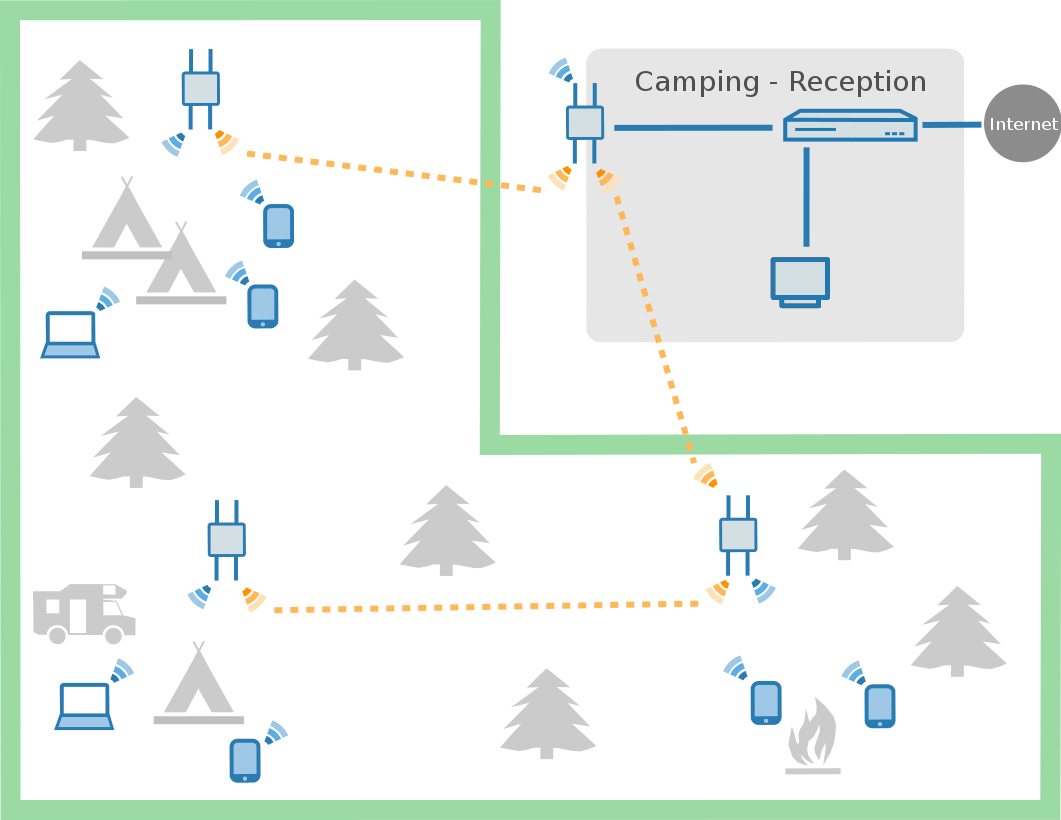
\includegraphics[width=1\columnwidth]{figures/camping.png}
    \caption{WDS deployment at a camping site. Typical scenario for using a WDS system instead of wired accesspoints.}
    \label{fig:camping}
  \end{figure}
  
\section{Motivation}
  AutoWDS provides such a system, but has problems with scalability and its throughput performance and connectivity failures leave somewhat to be desired.
  Our goal is therefore to optimize its performance so that it's up to its job of routing a large amounts of data through its wireless backbone and being resilient to simple link
  failures. We want to achieve this by utilizing multiple radios, channels and redundant links for establishing connections among the accesspoints, as using only a single
  channel places artificial limits on the achievable bandwidth one could obtain by exploiting more or the whole available spectrum.
  The problem we face doing this and our work will elaborate on, is that a good selection of links and channels is not trivial even for a moderately sized scenario.
  To tackle this issue we use centrally run greedy algorithms to give us a good solution to our problem for a static environment.
  
\section{Structure of Thesis}
  At first we will recall Terms and concepts used in this work. 
  This will be followed by taking a look at the requirements and restrictions a possible solution would have to deal with.
  In chapter 4 we will then review related work on this field and determine why those approached have not been facilitated.
  Finally in the following chapter we will describe then our algorithms for chosing a topology and channel assignment, closely ensued by the implementation of 
  the aforementioned. Here we will also give an example on how to run the code yourself for a certain scenario.
  In chapter 7 the whole procedure is evaluated in practice and compared to the basic version of AutoWDS.
  At last we summarize our findings and portray possible continuative paths we or someone else could follow.
